\section{Applications}

\subsection{Denoising}

\begin{description}
 \item[btkNLMDenoising] This program applies a non-local mean filter to a 3D image for denoising purpose. Usage: \texttt{-i input\_image\_filename -o output\_image\_filename}. The best results are usually obtained by using a mask (or a padding value).
\end{description}

\begin{description}
 \item[btkNLMDenoising4DImage] This program applies a non-local mean filter to each 3D image of a 4D image, for denoising purpose. Usage: \texttt{-i input\_image\_filename -o output\_image\_filename}. The best results are usually obtained by using a mask (or a padding value).
\end{description}


\subsection{Anatomical reconstruction}

\begin{description}
 \item[btkImageReconstruction] This program allows to obtain a
high-resolution image from a set of low-resolution images, typically
axial, coronal, and sagital acquisitions~\cite{Rousseau2006}. \\\\
Minimal usage: \texttt{btkImageReconstruction -i image1 $\cdots$ -i imageN -o
output}. 

Recommended usage: \texttt{btkImageReconstruction -i image1 $\cdots$ -i imageN
-m mask1 $\cdots$ -m maskN -o output --mask}. The use of a mask provide
better results since it allows an accuratelly estimation of the initial
transform, and constrains the registration to the region of interest.

The full list of optional parameters of the method can be obtained by
\texttt{btkImageReconstruction --help}

\end{description}

\begin{figure}[t]
\centering
\begin{tabular}{ccc}
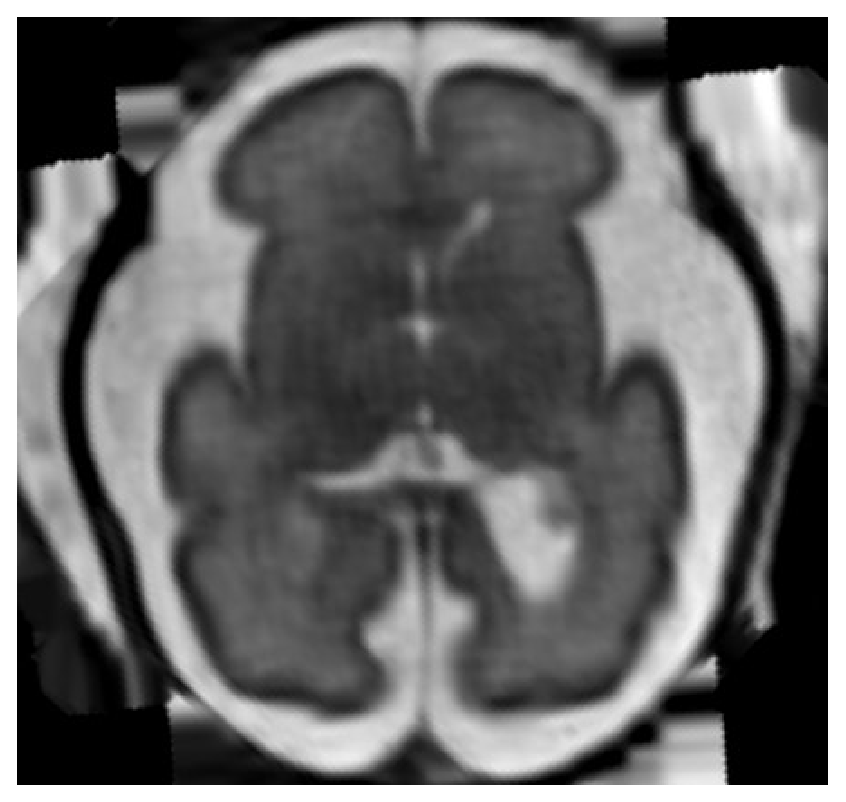
\includegraphics[width=0.3\columnwidth]{hr_axl.eps}&
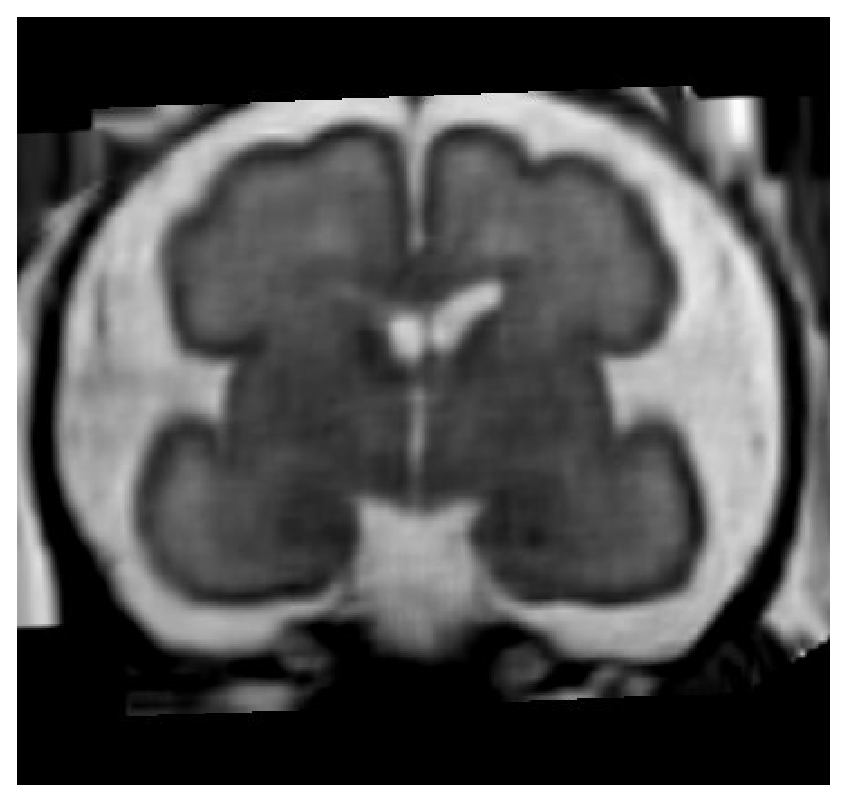
\includegraphics[width=0.3\columnwidth]{hr_cor.eps}&
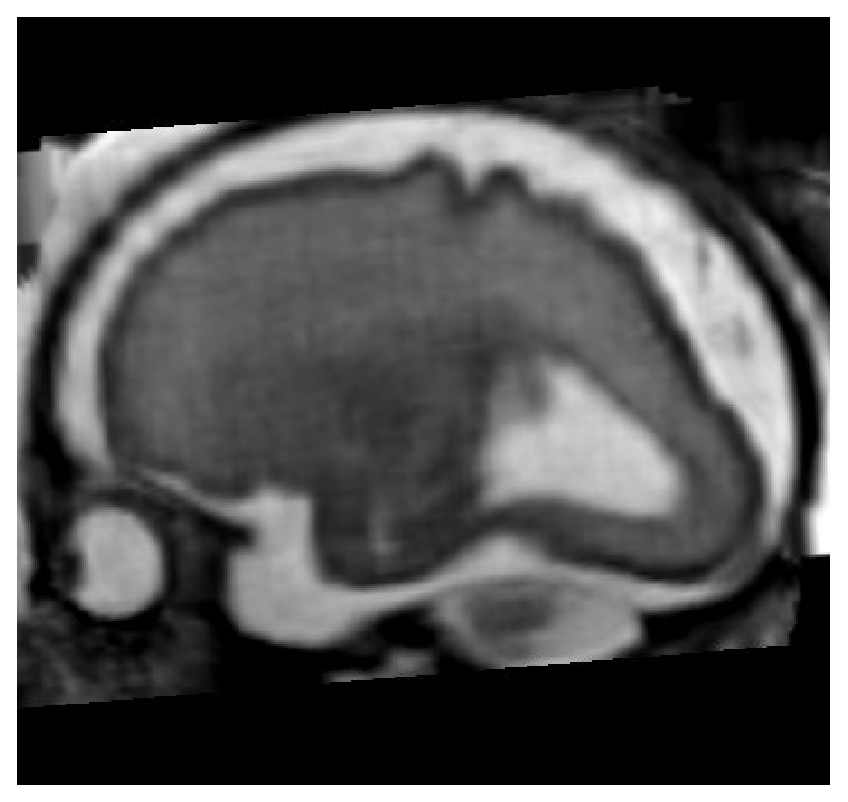
\includegraphics[width=0.3\columnwidth]{hr_sag.eps}\\
{(a)}&{(b)}&{(c)}\\
\end{tabular}
\caption{Example of an anatomical reconstruction of a fetal brain by using
\texttt{btkImageReconstruction}. (a) axial, (b) coronal, and (c) sagital view.}
\label{fig:reconstruction}
\end{figure}


\subsection{Tractography}

\begin{description}
 \item[btkTractography] This program performs a probabilistic tractography using a particle filtering. Usage: \texttt{-d dwi\_image\_filename -v dwi\_gradient\_vectors -m white\_matter\_mask -l seeds\_la\-bel\_image}.
\end{description}
